\documentclass[../main.tex]{subfiles}

\pagestyle{main}
\renewcommand{\chaptermark}[1]{\markboth{\chaptername\ \thechapter:\ #1}{}}
\setcounter{chapter}{8}

\begin{document}




\chapter{Methods of Integration}
\section{Basic Formulas}
\begin{itemize}
    \item \marginnote{6/30:}Useful, abstract info (that I already know) on what makes a student good at integating, e.g., integrating is an exercise in trial-and-error, but there are ways to increase your likelihood of being successful.
\end{itemize}



\section{Powers of Trigonometric Functions}
\begin{itemize}
    \item When integrating power functions, look for integral/derivative relationships, which may allow you to substitute $u$ and $\dd u$ at the same time.
    \begin{itemize}
        \item For example, when confronted with $\int \sin^nax\cos ax\dd{x}$, note that $\cos ax$ is almost the derivative of $\sin ax$, and choose $u=\sin ax$ and $\frac{\dd u}{a}=\cos ax\dd{x}$ to yield $\frac{1}{a}\int u^n\dd{u}$.
    \end{itemize}
    \item When integrating power functions, it may be possible to split the exponent into a product ($u^n=u^au^b$ where $a+b=n$) and work off of properties of one of the functions raised to a smaller exponent ($u^a$ may have properties that $u^n$ lacks).
    \begin{itemize}
        \item For example, when confronted with $\int \sin^3x\dd{x}$, recall that $\sin^2x$ has Pythagorean properties, and split the exponent.
        \begin{align*}
            \int\sin^3x\dd{x} &= \int\sin^2x\sin x\dd{x}\\
            &= \int\left( 1-\cos^2x \right)\sin x\dd{x}
            \intertext{Now we can use the previous property, since $\sin x$ and $\cos x$ have an integral/derivative relationship.}
            &= -\int\left( 1-u^2 \right)\dd{u}\\
            &= \int\left( u^2-1 \right)\dd{u}
        \end{align*}
        \item Note that this technique is applicable whenever an odd power of sine or cosine is to be integrated. For higher powers, consider the following.
        \begin{equation*}
            \int\cos^{2n+1}x\dd{x} = \int\left( \cos^2x \right)^n\cos x\dd{x}
            = \int\left( 1-\sin^2x \right)^n\cos x\dd{x}
            = \int\left( 1-u^2 \right)^n\dd{u}
        \end{equation*}
        Remember that $\left( 1-u^2 \right)^n$ can be expanded via the binomial theorem.
    \end{itemize}
    \item When integrating a composite trigonometric function, consider reducing it to a radical of powers of sines and cosines.
    \begin{itemize}
        \item For example, $\sec x\tan x = \frac{\sin x}{\cos^2x}$.
    \end{itemize}
    \item When integrating positive integer powers of $\tan x$, use either the base cases or the \textbf{reduction formula}.
    \begin{itemize}
        \item Begin by deriving a reduction formula.
        \begin{align*}
            \int\tan^nx\dd{x} &= \int\tan^{n-2}x\left( \sec^2x-1 \right)\dd{x}\\
            &= \int\tan^{n-2}\sec^2x\dd{x}-\int\tan^{n-2}x\dd{x}\\
            &= \frac{\tan^{n-1}x}{n-1}-\int\tan^{n-2}x\dd{x}
        \end{align*}
        Since the reduction formula decreases the exponent by 2, work out two base cases.
        \begin{gather*}
            \int\tan^0 x\dd{x} = \int\dd{x} = x+C\\
            \int\tan^1 x\dd{x} = \int\frac{\sin x}{\cos x}\dd{x}
            = -\int\frac{\dd u}{u}
            = -\ln|\cos x|+C
        \end{gather*}
        \item Note that the impetus for initially deriving such a formula was the search for a way to get $\sec^2x$ into the integrand, which can be done by splitting the exponent.
        \item This method can easily be adjusted to suit negative powers of $\tan x$ (positive powers of $\cot x$).
    \end{itemize}
    \item When integrating even powers of $\sec x$, either use the secant reduction formula, or split the exponent.
    \begin{itemize}
        \item We derive the following formula.
        \begin{align*}
            \int\sec^{2n}x\dd{x} &= \int\sec^{2n-2}x\sec^2x\dd{x}\\
            &= \int\left( 1+\tan^2x \right)^{n-1}\sec^2x\dd{x}\\
            &= \int\left( 1+u^2 \right)^{n-1}\dd{u}
        \end{align*}
    \end{itemize}
    \item When integrating secant (or cosecant) alone, produce $\frac{u'}{u}$ by multiplying the integrand by a clever form of 1.
    \begin{itemize}
        \item For example,
        \begin{align*}
            \int\sec x\dd{x} &= \int\sec x\cdot\frac{\sec x+\tan x}{\sec x+\tan x}\dd{x}\\
            &= \int\frac{\sec^2x+\sec x\tan x}{\sec x+\tan x}\\
            &= \ln|\sec x+\tan x|+C
        \end{align*}
    \end{itemize}
\end{itemize}



\section{Even Powers of Sines and Cosines}
\begin{itemize}
    \item When integrating the product of sines and cosines raised to powers where at least one exponent is a positive odd integer, split the exponent and use $u$-substitution.
    \begin{itemize}
        \item In effect, we wish to evaluate $\int\sin^mx\cos^nx\dd{x}$ where at least one of $m,n$ is a positive odd integer.
        \item For example, when confronted with $\int\cos^\frac{2}{3}x\sin^5x\dd{x}$, split the exponent of $\sin^5x$ and choose $u=\cos x$ and $-\dd u=\sin x\dd{x}$.
        \begin{equation*}
            \int\cos^\frac{2}{3}x\sin^5x\dd{x} = \int\cos^\frac{2}{3}x\left( 1-\cos^2x \right)^2\sin x\dd{x}
            = \int u^\frac{2}{3}\left( u^2-1 \right)\dd{u}
        \end{equation*}
    \end{itemize}
    \item When integrating the product of sines and cosines raised to powers where both exponents are even integers, begin by transforming it into a sum of either just sines \emph{or} just cosines raised to even integers. Then split the exponents and use one of the following formulas. It may be necessary to use these formulas multiple times. Use them until the problem has been reduced to a sum with only odd exponents.
    \begin{align*}
        \sin^2u &= \frac{1}{2}(1-\cos2u)&
        \cos^2u &= \frac{1}{2}(1+\cos2u)
    \end{align*}
    \begin{itemize}
        \item Note that \dq{these identities may be derived very quickly by adding or subtracting the equations [$\cos^2u+\sin^2u=1$ and $\cos^2u-\sin^2u=\cos2u$] and by dividing by two}{287}
        \item For example, when confronted with $\int\sin^2x\cos^4x\dd{x}$, begin by changing it to a case with only powers of cosine (chose to eliminate the sine function because it is raised to a lower exponent and, thus, will need less binomial expansion).
        \begin{align*}
            \int\sin^2x\cos^4x\dd{x} &= \int\left( 1-\cos^2x \right)\cos^4x\dd{x}\\
            &= \int\cos^4x\dd{x}-\int\cos^6x\dd{x}
            \intertext{Now split the exponents.}
            &= \int\left( \cos^2x \right)^2\dd{x}-\int\left( \cos^2x \right)^3\dd{x}
            \intertext{Employ the above formulas and use binomial expansion. If necessary, repeat (split the exponents, employ the above formulas, use binomial expansion) until only odd exponents remain (remember that 1 is an odd exponent).}
            &= \int\left( \frac{1}{2}(1+\cos2x) \right)^2\dd{x}-\int\left( \frac{1}{2}(1+\cos2x) \right)^3\dd{x}\\
            &= \frac{1}{4}\int\left( 1+2\cos2x+\cos^22x \right)\dd{x}\\
            &\qquad-\frac{1}{8}\int\left( 1+3\cos2x+3\cos^22x+\cos^32x \right)\dd{x}\\
            &= \frac{1}{4}\int\left( 1+2\cos2x+\frac{1}{2}(1+\cos4x) \right)\dd{x}\\
            &\qquad-\frac{1}{8}\int\left( 1+3\cos2x+\frac{3}{2}(1+\cos4x)+\cos^32x \right)\dd{x}
        \end{align*}
        These integrals may now be handled using previously discussed techniques.
    \end{itemize}
\end{itemize}



\section{Integrals With Terms \texorpdfstring{$\sqrt{a^2-u^2}$}{TEXT}, \texorpdfstring{$\sqrt{a^2+u^2}$}{TEXT}, \texorpdfstring{$\sqrt{u^2-a^2}$}{TEXT}, \texorpdfstring{$a^2+u^2$}{TEXT}, \texorpdfstring{$a^2-u^2$}{TEXT}}
\begin{itemize}
    \item When integrating a radical that resembles the derivative of an inverse trig function, we may factor out the issue so as to make the integral resemble one of the known formulas.
    \begin{itemize}
        \item For example, when confronted with $\int\frac{\dd u}{a^2+u^2}$, divide the $a^2$ term out of the denominator and integrate with respect to $\frac{u}{a}$\footnote{\cite{bib:Thomas} uses differentials with more complex functions than a single variable quite often. It's not something I've seen before, but it's something I should get used to (and it does make sense if you think about it --- it's just an extension of the underlying concept of separation of variables integration).}.
        \begin{align*}
            \int\frac{\dd u}{a^2+u^2} &= \frac{1}{a^2}\int\frac{\dd u}{1+\left( \frac{u}{a} \right)^2}\\
            &= \frac{1}{a^2}\int\frac{a\dd{\left( \frac{u}{a} \right)}}{1+\left( \frac{u}{a} \right)^2}\\
            &= \frac{1}{a}\tan^{-1}\frac{u}{a}+C
        \end{align*}
        \item However, this method is partially flawed in that it relies on having memorized the derivatives of the inverse trig functions, i.e., it is not terribly analytical. This shortcoming will now be addressed with a new, more general technique.
    \end{itemize}
    \item The new method leans heavily on the following three identities.
    \begin{align*}
        1-\sin^2\theta &= \cos^2\theta&
        1+\tan^2\theta &= \sec^2\theta&
        \sec^2\theta-1 &= \tan^2\theta
    \end{align*}
    \begin{itemize}
        \item With the help of these identities, it is possible to\dots
        \begin{enumerate}
            \item use $u=a\sin\theta$ to replace $a^2-u^2$ with $a^2\cos^2\theta$;
            \item use $u=a\tan\theta$ to replace $a^2+u^2$ with $a^2\sec^2\theta$;
            \item use $u=a\sec\theta$ to replace $u^2-a^2$ with $a^2\tan^2\theta$.
        \end{enumerate}
        \begin{figure}[h!]
            \centering
            \begin{subfigure}[b]{0.3\linewidth}
                \centering
                \begin{tikzpicture}[
                    every node/.style={black}
                ]
                    \footnotesize
                    \draw [ylx,thick]
                        (0,0) coordinate (B) -- node[below]{$\cos\theta$}
                        (2,0) coordinate (A) -- node[right]{$\sin\theta$}
                        (2,1.2) coordinate (C) -- node[above]{$1$}
                        cycle
                    ;
                    \begin{scope}[on background layer]
                        \pic[pic text={$\theta$},draw,thin,angle radius=8mm,angle eccentricity=1.2]{angle};
                    \end{scope}
                \end{tikzpicture}
                \caption{$\cos^2\theta+\sin^2\theta=1$.}
                \label{fig:trigIdentitiesa}
            \end{subfigure}
            \begin{subfigure}[b]{0.3\linewidth}
                \centering
                \begin{tikzpicture}[
                    every node/.style={black}
                ]
                    \footnotesize
                    \draw [ylx,thick]
                        (0,0) coordinate (B) -- node[below]{$1$}
                        (2,0) coordinate (A) -- node[right]{$\tan\theta$}
                        (2,1.2) coordinate (C) -- node[above,xshift=-2mm]{$\sec\theta$}
                        cycle
                    ;
                    \begin{scope}[on background layer]
                        \pic[pic text={$\theta$},draw,thin,angle radius=8mm,angle eccentricity=1.2]{angle};
                    \end{scope}
                \end{tikzpicture}
                \caption{$1+\tan^2\theta=\sec^2\theta$.}
                \label{fig:trigIdentitiesb}
            \end{subfigure}
            \begin{subfigure}[b]{0.3\linewidth}
                \centering
                \begin{tikzpicture}[
                    every node/.style={black}
                ]
                    \footnotesize
                    \draw [ylx,thick]
                        (0,0) coordinate (B) -- node[below]{$\cot\theta$}
                        (2,0) coordinate (A) -- node[right]{$1$}
                        (2,1.2) coordinate (C) -- node[above,xshift=-2mm]{$\csc\theta$}
                        cycle
                    ;
                    \begin{scope}[on background layer]
                        \pic[pic text={$\theta$},draw,thin,angle radius=8mm,angle eccentricity=1.2]{angle};
                    \end{scope}
                \end{tikzpicture}
                \caption{$\cot^2\theta+1=\csc^2\theta$.}
                \label{fig:trigIdentitiesc}
            \end{subfigure}
            \caption{Geometric rationale for the trigonometric identities.}
            \label{fig:trigIdentities}
        \end{figure}
        \begin{figure}[h!]
            \centering
            \begin{subfigure}[b]{0.3\linewidth}
                \centering
                \begin{tikzpicture}[
                    every node/.style={black}
                ]
                    \footnotesize
                    \draw [ylx,thick]
                        (0,0) coordinate (B) -- node[below]{$\color{white}a$}
                        (2,0) coordinate (A) -- node[right]{$u$}
                        (2,1.2) coordinate (C) -- node[above]{$a$}
                        cycle
                    ;
                    \begin{scope}[on background layer]
                        \pic[pic text={$\theta$},draw,thin,angle radius=8mm,angle eccentricity=1.2]{angle};
                    \end{scope}
                \end{tikzpicture}
                \caption{$\sqrt{a^2-u^2}=a\cos\theta$\\ $u=a\sin\theta$.}
                \label{fig:trigSubstitutionsa}
            \end{subfigure}
            \begin{subfigure}[b]{0.3\linewidth}
                \centering
                \begin{tikzpicture}[
                    every node/.style={black}
                ]
                    \footnotesize
                    \draw [ylx,thick]
                        (0,0) coordinate (B) -- node[below]{$a$}
                        (2,0) coordinate (A) -- node[right]{$u$}
                        (2,1.2) coordinate (C) --
                        cycle
                    ;
                    \begin{scope}[on background layer]
                        \pic[pic text={$\theta$},draw,thin,angle radius=8mm,angle eccentricity=1.2]{angle};
                    \end{scope}
                \end{tikzpicture}
                \caption{$\sqrt{u^2+a^2}=a\sec\theta$\\ $u=a\tan\theta$.}
                \label{fig:trigSubstitutionsb}
            \end{subfigure}
            \begin{subfigure}[b]{0.3\linewidth}
                \centering
                \begin{tikzpicture}[
                    every node/.style={black}
                ]
                    \footnotesize
                    \draw [ylx,thick]
                        (0,0) coordinate (B) -- node[below]{$a$}
                        (2,0) coordinate (A) --
                        (2,1.2) coordinate (C) -- node[above]{$u$}
                        cycle
                    ;
                    \begin{scope}[on background layer]
                        \pic[pic text={$\theta$},draw,thin,angle radius=8mm,angle eccentricity=1.2]{angle};
                    \end{scope}
                \end{tikzpicture}
                \caption{$\sqrt{u^2-a^2}=a\tan\theta$\\ $u=a\sec\theta$.}
                \label{fig:trigSubstitutionsc}
            \end{subfigure}
            \caption{Geometric rationale for the trigonometric substitutions.}
            \label{fig:trigSubstitutions}
        \end{figure}
        \item These identities and substitutions can be easily remembered by thinking of the Pythagorean theorem in conjunction with Figures \ref{fig:trigIdentities} and \ref{fig:trigSubstitutions}, respectively.
    \end{itemize}
    \item We may now evaluate inverse trig integrals analytically.
    \begin{itemize}
        \item For example, when confronted with $\int\frac{\dd u}{a^2+u^2}$, choose $u=a\tan\theta$ and $\dd u=a\sec^2\theta\dd{\theta}$.
        \begin{align*}
            \int\frac{\dd u}{a^2+u^2} &= \int\frac{a\sec^2\theta\dd{\theta}}{a^2+(a\tan\theta)^2}\\
            &= \int\frac{a\sec^2\theta}{a^2\left( 1+\tan^2\theta \right)}\dd{\theta}\\
            &= \frac{1}{a}\int\frac{\sec^2\theta}{\sec^2\theta}\dd{\theta}\\
            &= \frac{1}{a}\int\dd{\theta}\\
            &= \frac{1}{a}\theta+C
            \intertext{At this point, solve $u=a\tan\theta$ for $\theta$ and substitute.}
            &= \frac{1}{a}\tan^{-1}\frac{u}{a}+C
        \end{align*}
        \item Some integrals will simplify to have a plus/minus in the denominator, leading to two possible solutions. However, there are sometimes ways to isolate a single solution.
        \begin{itemize}
            \item For example, $\int\frac{\dd u}{\sqrt{a^2-u^2}}=\int\frac{a\cos\theta\dd{\theta}}{\pm a\cos\theta}=\pm\theta+C$. However, when we consider the fact that $\theta=\sin^{-1}\frac{u}{a}$, we know that $\theta\in\left[ -\frac{\pi}{2},\frac{\pi}{2} \right]$ (because inverse sine is not arcsine, and inverse sine is only defined over the principal branch of sine). Thus, since $\theta\in\left[ -\frac{\pi}{2},\frac{\pi}{2} \right]$, $\cos\theta\in[0,1]$, i.e., is always positive. Thus, we choose $\int\frac{\dd u}{\sqrt{a^2-u^2}}=+\theta+C=\sin^{-1}\frac{u}{a}+C$ as our one solution.
            \item For example, $\int\frac{\dd u}{\sqrt{u^2-a^2}}$ equals $\ln\left| \frac{u}{a}+\frac{\sqrt{u^2-a^2}}{a} \right|+C$ or $-\ln\left| \frac{u}{a}-\frac{\sqrt{u^2-a^2}}{a} \right|+C$ depending on whether $\tan\theta$ is positive or negative. But it can be shown algebraically that the two solutions are actually equal:
            \begin{align*}
                -\ln\left| \frac{u}{a}-\frac{\sqrt{u^2-a^2}}{a} \right| &= \ln\left| \frac{a}{u-\sqrt{u^2-a^2}} \right|\\
                &= \ln\left| \frac{a\left( u+\sqrt{u^2-a^2} \right)}{\left( u-\sqrt{u^2-a^2} \right)\left( u+\sqrt{u^2-a^2} \right)} \right|\\
                &= \ln\left| \frac{a\left( u+\sqrt{u^2-a^2} \right)}{a^2} \right|\\
                &= \ln\left| \frac{u}{a}+\frac{\sqrt{u^2-a^2}}{a} \right|
            \end{align*}
            Thus, we have $\ln\left| \frac{u}{a}+\frac{\sqrt{u^2-a^2}}{a} \right|+C$ as the one solution\footnote{Note that we could choose to use the other solution, but we choose this one because it's "simpler" (it uses addition instead of subtraction).}.
        \end{itemize}
        \item Some integrals will have extraneous constants that can be combined with $C$ to simplify the \emph{indefinite} integral.
        \begin{itemize}
            \item Continuing with the above example,
            \begin{align*}
                \int\frac{\dd u}{\sqrt{u^2-a^2}} &= \ln\left| \frac{u}{a}+\frac{\sqrt{u^2-a^2}}{a} \right|+C\\
                &= \ln\left| u+\sqrt{u^2-a^2} \right|-\ln|a|+C\\
                &= \ln\left| u+\sqrt{u^2-a^2} \right|+C
            \end{align*}
        \end{itemize}
    \end{itemize}
    \item When integrating an inverse trig integral with excess polynomial terms, look to transform it into a (power of a) trig integral problem.
    \begin{itemize}
        \item For example, when confronted with $\int\frac{x^2\dd{x}}{\sqrt{9-x^2}}$, treat it as a case of $a^2-u^2$, but substitute the trig expression into the $x^2$ term in the numerator, too.
        \begin{equation*}
            \int\frac{x^2\dd{x}}{\sqrt{9-x^2}} = \int\frac{9\sin^2\theta\cdot 3\cos\theta\dd{\theta}}{3\cos\theta}
            = 9\int\sin^2\theta\dd{\theta}
        \end{equation*}
        This integral may now be handled using previously discussed techniques.
    \end{itemize}
    \item Many inverse trig integrals can also be evaluated hyperbolically, making use of the following three identities.
    \begin{align*}
        \cosh^2\theta-1 &= \sinh^2\theta&
        1-\tanh^2\theta &= \sech^2\theta&
        1+\sinh^2\theta &= \cosh^2\theta
    \end{align*}
    \begin{itemize}
        \item With the help of these identities, it is possible to\dots
        \begin{enumerate}
            \item use $u=a\tanh\theta$ to replace $a^2-u^2$ with $a^2\sech^2\theta$;
            \item use $u=a\sinh\theta$ to replace $a^2+u^2$ with $a^2\cosh^2\theta$;
            \item use $u=a\cosh\theta$ to replace $u^2-a^2$ with $a^2\sinh^2\theta$.
        \end{enumerate}
    \end{itemize}
\end{itemize}



\section{Integrals With \texorpdfstring{$ax^2+bx+c$}{TEXT}}
\begin{itemize}
    \item When integrating composite functions where the inner function is a binomial, look to factor said binomial.
    \begin{itemize}
        \item The general quadratic $f(x)=ax^2+bx+c$, $a\neq 0$, can be reduced to the form $a\left( u^2+B \right)$ by completing the square and choosing $u=x+\frac{b}{2a}$ and $B=\frac{4ac-b^2}{4a^2}$:
        \begin{align*}
            ax^2+bx+c &= a\left( x^2+\frac{b}{a}x \right)+c\\
            &= a\left( x^2+\frac{b}{a}x+\frac{b^2}{4a^2} \right)+c-\frac{b^2}{4a}\\
            &= a\left( \left( x+\frac{b}{2a} \right)^2+\frac{4ac-b^2}{4a^2} \right)
        \end{align*}
    \end{itemize}
    \item When integrating the square root of a binomial, or some similarly tricky function of a binomial, we can transform the binomial into a form such that it will suit one of the inverse trig integrals.
    \begin{itemize}
        \item Since it would lead to complex numbers, we disregard cases where $a\left( u^2+B \right)$ is negative, i.e., we focus on cases where (1) $a$ is positive, and (2) $a,B$ are both negative.
        \item That being said, if it is an odd root ($\sqrt[3]{x}$, $\sqrt[5]{x}$, etc.), the sign doesn't matter.
        \item For example, when confronted with $\int\frac{(x+1)\dd{x}}{\sqrt{2x^2-6x+4}}$, begin by factoring the binomial\footnote{Note that, in place of inspection, we could use the general form factorization derived above.}.
        \begin{equation*}
            2x^2-6x+4 = 2\left( x^2-3x \right)+4
            = 2\left( x-\frac{3}{2} \right)^2-\frac{1}{2}
            = 2\left( u^2-a^2 \right)
        \end{equation*}
        Note that $u=x-\frac{3}{2}$ and $a=\frac{1}{2}$. We can now return to the integral, which we shall reformulate in terms of $u$ in its entirety.
        \begin{align*}
            \int\frac{(x+1)\dd{x}}{\sqrt{2x^2-6x+4}} &= \int\frac{\left( u+\frac{5}{2} \right)\dd{u}}{\sqrt{2\left( u^2-a^2 \right)}}
            \intertext{Split it into two separate integrals and factor out the constants.}
            &= \frac{1}{\sqrt{2}}\int\frac{u\dd{u}}{\sqrt{u^2-a^2}}+\frac{5}{2\sqrt{2}}\int\frac{\dd u}{\sqrt{u^2-a^2}}
            \intertext{The right integral is a straight-up inverse trig integral. The left one, however, needs something special. It could be dealt with as previously discussed by substituting $u=a\tan\theta$ for all instances of $u$ and evaluating it is a more complex trig integral in $\theta$. However, for the sake of showing a different technique, we will choose $z=u^2-a^2$ and $\frac{1}{2}\dd z=u\dd{u}$ and treat it as a power function in $z$.}
            &= \frac{1}{2\sqrt{2}}\int\frac{\dd{z}}{\sqrt{z}}+\frac{5}{2\sqrt{2}}\ln\left| u+\sqrt{u^2-a^2} \right|+C_2\\
            &= \frac{1}{2\sqrt{2}}\int z^{-\frac{1}{2}}\dd{z}+\frac{5}{2\sqrt{2}}\ln\left| u+\sqrt{u^2-a^2} \right|+C_2\\
            &= \frac{1}{\sqrt{2}}z^\frac{1}{2}+C_1+\frac{5}{2\sqrt{2}}\ln\left| u+\sqrt{u^2-a^2} \right|+C_2
            \intertext{Return all of the substitutions and combine the constants of integration.}
            &= \sqrt{\frac{u^2-a^2}{2}}+\frac{5}{2\sqrt{2}}\ln\left| u+\sqrt{u^2-a^2} \right|+C\\
            &= \sqrt{\frac{x^2-3x+2}{2}}+\frac{5}{2\sqrt{2}}\ln\left| x-\frac{3}{2}+\sqrt{x^2-3x+2} \right|+C
        \end{align*}
    \end{itemize}
\end{itemize}



\section{Integration by the Method of Partial Fractions}
\begin{itemize}
    \item \marginnote{7/1:}\textbf{Method of Partial Fractions}: The process of \dq{split[ting] a fraction into a sum of fractions having simpler denominators}{294}
    \item If we wish to split a rational fraction $\frac{f(x)}{g(x)}$ into a sum of simpler fractions, then\dots
    \begin{itemize}
        \item \dq{The degree of $f(x)$ should be less than the degree of $g(x)$. If this is not the case, we first perform a long division, then work with the remainder term. This remainder can always be put into the required form}{294}
        \item \dq{The factors of $g(x)$ should be known. Theoretically, any polynomial $g(x)$ with real coefficient can be expressed as a product of real linear and quadratic factors. In practice, it may be difficult to perform the factorization}{294}
    \end{itemize}
    \item If $x-r$ is a linear factor of $g(x)$ and $(x-r)^m$ is the highest power of $x-r$ that divides $g(x)$, then, to this factor, assign the sum of $m$ partial fractions
    \begin{equation*}
        \frac{A_1}{x-r}+\frac{A_2}{(x-r)^2}+\cdots+\frac{A_m}{(x-r)^m}
    \end{equation*}
    \begin{itemize}
        \item If $x^2+px+q$ is a quadratic factor\footnote{A binomial factor, the factoring of which into linear factors would introduce complex numbers.} of $g(x)$ and $\left( x^2+px+q \right)^n$ is the highest power of $x^2+px+q$ that divides $g(x)$, then, to this factor, assign the sum of $n$ partial fractions
    \end{itemize}
    \begin{equation*}
        \frac{B_1x+C_1}{x^2+px+q}+\frac{B_2x+C_2}{\left( x^2+px+q \right)^2}+\cdots+\frac{B_nx+C_n}{\left( x^2+px+q \right)^n}
    \end{equation*}
    \begin{itemize}
        \item Continue, as necessary, to higher degree factors of $g(x)$ (although this caveat is not addressed by \cite{bib:Thomas}).
    \item Notice how the degree of the polynomial in the numerator of the partial fractions will be at most one less than the degree of the denominator.
    \end{itemize}
    \item Any rational function integrated via the method of partial fractions can be reduced to the problem of evaluating the following two types of integrals.
    \begin{align*}
        \int\frac{\dd x}{(x-r)^h}&&
        \int\frac{(ax+b)\dd{x}}{\left( x^2+px+q \right)^k}
    \end{align*}
    \begin{itemize}
        \item The left integral, with the substitution $z=x-r$ and $\dd{z}=\dd{x}$, becomes a power integral.
        \item The right integral, after completing the square in the denominator, substituting, and splitting into two fractions by the numerator, becomes a pair of inverse trig substitution integrals.
    \end{itemize}
    \item With the method of partial fractions, there is a new way to integrate $\sec\theta$.
    \begin{align*}
        \int\sec\theta\dd{\theta} &= \int\frac{\dd\theta}{\cos\theta}\\
        &= \int\frac{\cos\theta\dd{\theta}}{\cos^2\theta}\\
        &= \int\frac{\dd x}{1-x^2}\\
        &= \int\frac{0.5}{1+x}\dd{x}+\int\frac{0.5}{1-x}\dd{x}\\
        &= \frac{1}{2}\ln|1+x|-\frac{1}{2}\ln|1-x|+C\\
        &= \frac{1}{2}\ln\left| \frac{1+x}{1-x} \right|+C\\
        &= \ln\sqrt{\frac{1+\sin\theta}{1-\sin\theta}}+C
    \end{align*}
    \begin{itemize}
        \item Note that $\ln\sqrt{\frac{1+\sin\theta}{1-\sin\theta}}+C$ is equivalent to the previously derived form:
        \begin{align*}
            \sqrt{\frac{1+\sin\theta}{1-\sin\theta}} &= \sqrt{\frac{(1+\sin\theta)^2}{1-\sin^2\theta}}\\
            &= \left| \frac{1+\sin\theta}{\cos\theta} \right|\\
            &= |\sec\theta+\tan\theta|
        \end{align*}
    \end{itemize}
\end{itemize}



\section{Integration by Parts}
\begin{itemize}
    \item This is the second general method of integration (the first being substitution).
    \item It relies on the following formulas for indefinite and definite integrals, respectively.
    \begin{align*}
        \int u\dd{v} &= uv-\int v\dd{u}+C&
        \int_{(1)}^{(2)}u\dd{v} &= uv\Big]_{(1)}^{(2)}-\int_{(1)}^{(2)}v\dd{u}
    \end{align*}
    \begin{itemize}
        \item The indefinite integral formula can be derived from the differential of a product rule as follows.
        \begin{align*}
            \dd{(uv)} &= u\dd{v}+v\dd{u}\\
            u\dd{v} &= \dd{(uv)}-v\dd{u}\\
            \int u\dd{v} &= uv-\int v\dd{u}+C
        \end{align*}
        \begin{figure}[h!]
            \centering
            \begin{tikzpicture}[
                scale=1.6,
                every node/.style={black}
            ]
                \footnotesize
                \fill [gay] (0,0.945) node[left]{$u_1$} -- plot [domain=0.7:2,smooth] (\x,{1.3+1.2*sin((\x-1) r)}) -- (0,2.31) node[left]{$u_2$};
                \fill [yly] (0.7,0) node[below]{$v_1$} -- plot [domain=0.7:2,smooth] (\x,{1.3+1.2*sin((\x-1) r)}) -- (2,0) node[below]{$v_2$};
                \draw [thick,ylx] plot [domain=0.3:2.3,smooth] (\x,{1.3+1.2*sin((\x-1) r)}) node[right]{$u=f(v)$};

                \draw [-stealth] (-0.35,0) -- (3,0) node[right]{$v$};
                \draw [-stealth] (0,-0.4) -- (0,3) node[above]{$u$};

                \node [below left] {$O$};
                \node at (1.35,0.7) {$\int u\dd{v}$};
                \node at (0.53,1.65) {$\int v\dd{u}$};
            \end{tikzpicture}
            \caption{Geometric rationale for definite integration by parts.}
            \label{fig:integrationByParts}
        \end{figure}
        \item The definite integral formula can be thought of as an adjustment of the above, or it can be conceived geometrically: In Figure \ref{fig:integrationByParts}, $\int_{(1)}^{(2)}u\dd{v}$ is the yellow area, which is clearly equivalent to the total area\footnote{Note that $uv\big]_{(1)}^{(2)}=u_2v_2-u_1v_1$, the latter of which, as the difference of two rectangles, clearly represents the total shaded area.} $uv\big]_{(1)}^{(2)}$ minus the grey area $\int_{(1)}^{(2)}v\dd{u}$.
    \end{itemize}
    \item Since $\int\dd v=v+C_1$, $\int u\dd{v}$ actually equals $u(v+C_1)-\int(v+C_1)\dd{u}$. However, since
    \begin{align*}
        u(v+C_1)-\int(v+C_1)\dd{u} &= uv+C_1u-\int v\dd{u}-\int C_1\dd{u}\\
        &= uv-\int v\dd{u}
    \end{align*}
    it is customary to drop the first constant of integration.
    \begin{itemize}
        \item That being said, it is sometimes useful --- when evaluating $\int\ln(x+1)\dd{x}=\ln(x+1)(x+C_1)-\int\frac{x+C_1}{x+1}\dd{x}$, being able to choose $C_1=1$ greatly simplifies the second integral.
    \end{itemize}
    \item When integrating an inverse trig function, consider using integration by parts.
    \begin{itemize}
        \item For example, when confronted with $\int\tan^{-1}x\dd{x}$, integration by parts turns it into an inverse trig derivative problem.
        \begin{equation*}
            \int\tan^{-1}x\dd{x} = x\tan^{-1}x-\int\frac{x\dd{x}}{1+x^2}
        \end{equation*}
    \end{itemize}
    \item When attempting integration by parts, don't be afraid to use it multiple times.
    \begin{itemize}
        \item For example, when confronted with $\int x^2\e[x]\dd{x}$, use integration by parts twice.
        \begin{align*}
            \int x^2\e[x]\dd{x} &= x^2\e[x]-\int 2x\e[x]\dd{x}\\
            &= x^2\e[x]-\left( 2x\e[x]-\int 2\e[x]\dd{x} \right)
        \end{align*}
    \end{itemize}
    \item When attempting integration by parts, look for the original integral showing up again --- if it does, combine like terms.
    \item When integrating powers of $\cos x$, consider using a reduction formula.
    \begin{itemize}
        \item Begin by deriving a reduction formula (this will involve splitting the exponent!).
        \begin{align*}
            \int\cos^nx\dd{x} &= \int\cos^{n-1}x\cos x\dd{x}\\
            &= \cos^{n-1}x\sin x+(n-1)\int\cos^{n-2}x\sin^2x\dd{x}\\
            &= \cos^{n-1}x\sin x+(n-1)\int\cos^{n-2}x\dd{x}-(n-1)\int\cos^nx\dd{x}\\
            (1+(n-1))\int\cos^nx\dd{x} &= \cos^{n-1}x\sin x+(n-1)\int\cos^{n-2}x\dd{x}\\
            \int\cos^nx\dd{x} &= \frac{\cos^{n-1}x\sin x}{n}+\frac{n-1}{n}\int\cos^{n-2}x\dd{x}
        \end{align*}
        Since the reduction formula decreases the exponent by 2, work out two base cases.
        \begin{gather*}
            \int\cos^0x\dd{x} = x+C\\
            \int\cos^1x\dd{x} = \sin x+C
        \end{gather*}
    \end{itemize}
    \item When integrating powers of $\sin x$, consider using a reduction formula.
    \begin{equation*}
        \int\sin^nx\dd{x} = -\frac{\sin^{n-1}x\cos x}{n}+\frac{n-1}{n}\int\sin^{n-2}x\dd{x}
    \end{equation*}
\end{itemize}



\section{Integration of Rational Functions of \texorpdfstring{$\sin x$}{TEXT} and \texorpdfstring{$\cos x$}{TEXT}, and Other Trigonometric Integrals}
\begin{itemize}
    \item \dq{It has been discovered that the substitution $z=\tan\frac{x}{2}$ enables one to reduce the problem of integrating any rational function of $\sin x$ and $\cos x$ to a problem involving a rational function of $z$. This in turn can be integrated by the method of partial fractions}{300}
    \begin{itemize}
        \item However, this substitution should be used only as a last resort --- the associated algebra is often quite cumbersome.
    \end{itemize}
    \item To increase the ease of use for this substitution, it will help to derive three results.
    \begin{align*}
        \cos x &= \frac{1-z^2}{1+z^2}&
        \sin x &= \frac{2z}{1+z^2}&
        \dd x &= \frac{2\dd{z}}{1+z^2}
    \end{align*}
    \item \dq{The following types of integrals\dots arise in connection with alternating-current theory, heat transfer problems, bending of beams, cable stress analysis in suspension bridges, and many other places where trigonometric series (or Fourier series) are applied to problems in mathematics, science, and engineering}{301}
    \begin{align*}
        \int\sin mx\sin nx\dd{x}&&
        \int\sin mx\cos nx\dd{x}&&
        \int\cos mx\cos nx\dd{x}
    \end{align*}
    \item When confronted with one of these integrals, integration by parts may be used. However, using one of the following three identities will be more simple.
    \begin{align*}
        \sin mx\sin nx &= \frac{1}{2}(\cos(m-n)x-\cos(m+n)x)\\
        \sin mx\cos nx &= \frac{1}{2}(\sin(m-n)x+\sin(m+n)x)\\
        \cos mx\cos nx &= \frac{1}{2}(\cos(m-n)x+\cos(m+n)x)
    \end{align*}
    \begin{itemize}
        \item Note that \dq{these identities follow at once from $\cos(A+B)=\cos A\cos B-\sin A\sin B$, $\cos(A-B)=\cos A\cos B+\sin A\sin B$, and $\sin(A+B)=\sin A\cos B+\cos A\sin B$, $\sin(A-B)=\sin A\cos B-\cos A\sin B$}{301}
    \end{itemize}
\end{itemize}



\section{Further Substitutions}
\begin{itemize}
    \item \dq{Some integrals involving fractional powers of the variable $x$ may be simplified by substituting $x=z^n$, where $n$ is the least common multiple of the denominators of the exponents}{302}
    \begin{itemize}
        \item For example, $\int\frac{\sqrt{x}\dd{x}}{1+\sqrt[4]{x}}$ can be simplified by taking $x=z^4$.
    \end{itemize}
    \item \dq{Even when it is not clear at the start that a substitution will work, it is advisable to try one that seems reasonable and pursue it until it either gives results or appears to make matters worse. In the latter case, try something else! Sometimes a chain of substitutions $u=f(x)$, $v=g(u)$, $z=h(v)$, and so on, will produce results when it is by no means obvious that this will work}{302}
    \item \dq{The criterion of success is whether the new integrals so obtained appear to be simpler than the original integral. Here it is handy to remember that any rational function of $x$ can be integrated by the method of partial fractions and that any rational function of $\sin x$ and $\cos x$ can be integrated by using the substitution $z=\tan\frac{x}{2}$. If we can reduce a given integral to one of these types, we then know how to finish the job}{302}
    \item To evaluate a definite integral after a (series of) substitution(s), either return the substitution(s) and keep the bounds or keep the substitution(s) and determine new bounds based on the new variable of integration.
    \begin{itemize}
        \item For example, if $z^2=\frac{1+x}{1-x}$ and $x\in[-1,1]$, then $z\in[0,\infty)$. And if $z=\tan\theta$, then $\theta\in\left[ 0,\frac{\pi}{2} \right]$.
    \end{itemize}
\end{itemize}



\section{Improper Integrals}
\begin{itemize}
    \item \textbf{Improper integral}: An integral of the form $\int_a^b f(x)\dd{x}$ where some $x\in[a,b]$ is infinite, and/or one or both of $a,b$ are infinite in magnitude.
    \begin{figure}[h!]
        \centering
        \begin{subfigure}[b]{0.48\linewidth}
            \centering
            \begin{tikzpicture}[xscale=2.5,yscale=1.5]
                \footnotesize
                \fill [yly] plot [domain=-1:0.73,samples=100,smooth] (\x,{((1+\x)/(1-\x))^0.5}) -- (0.73,0) node[below,black]{$b$};

                \draw [-stealth] (-1.3,0) -- (1.3,0) node[right]{$x$};
                \draw [-stealth] (0,-0.4) -- (0,3.3) node[above]{$y$};
                \draw (-1,0.1) -- ++(0,-0.2) node[below]{$-1$};
                \draw (1,3.3) -- ++(0,-3.4) node[below]{$1$};
                \foreach \y in {1,2} {
                    \draw [xscale=0.6] (0.1,\y) -- ++(-0.2,0) node[left]{$\y$};
                }

                \draw [ylx,thick] plot [domain=-1:0.833,samples=100,smooth] (\x,{((1+\x)/(1-\x))^0.5});

                \node [below left] {$0$};
                \node at (-0.7,1.5) {$y=\sqrt{\dfrac{1+x}{1-x}}$};
            \end{tikzpicture}
            \caption{With respect to $x$.}
            \label{fig:impropera}
        \end{subfigure}
        \begin{subfigure}[b]{0.48\linewidth}
            \centering
            \begin{tikzpicture}[xscale=2.5,yscale=1.5]
                \footnotesize
                \fill [yly] (0.3,1.363) coordinate (P) rectangle (1,1.2);

                \draw [-stealth] (-1.3,0) -- (1.3,0) node[right]{$x$};
                \draw [-stealth] (0,-0.4) -- (0,3.3) node[above]{$y$};
                \draw (-1,0.1) -- ++(0,-0.2) node[below]{$(-1,0)$};
                \draw (1,3.3) -- ++(0,-3.4) node[below]{$(1,0)$};

                \draw ($(P)+(0,-0.2)$) -- ++(0,-0.3);
                \draw [<->] ($(P)+(0,-0.35)$) -- node[fill=white,inner sep=1.5pt]{$1-x$} ++(0.7,0);
                \draw ($(P)+(0.72,0)$) -- ++(0.16,0) (1.02,1.2) -- ++(0.16,0);
                \draw [->] (1.1,1.6) node[above]{$\dd y$} -- (P -| 1.1,0);
                \draw [->] (1.1,0.963) -- (1.1,1.2);

                \node [below left] {$O$};
                \node at (-0.7,1.5) {$x=\dfrac{y^2-1}{y^2+1}$};
                \node at (0.5,0.3) {$\dd{A}=(1-x)\dd{y}$};
                \node at (0.25,2) {$P(x,y)$}
                    edge (P)
                ;

                \draw [ylx,thick] plot [domain=-1:0.833,samples=100,smooth] (\x,{((1+\x)/(1-\x))^0.5});
            \end{tikzpicture}
            \caption{With respect to $y$.}
            \label{fig:improperb}
        \end{subfigure}
        \caption{Defining improper integrals.}
        \label{fig:improper}
    \end{figure}
    \item Say we wish to evaluate $\int_{-1}^1\sqrt{\frac{1+x}{1-x}}\dd{x}$, knowing that the integrand approaches $\infty$ as $x\to 1$ (see Figure \ref{fig:impropera}). Well, if the upper bound $b$ is some value slightly \emph{less than} 1, we \emph{can} evaluate the integral. Thus evaluating the original integral becomes a problem of evaluating
    \begin{equation*}
        \lim_{b\to 1^-}\int_{-1}^b\sqrt{\frac{1+x}{1-x}}\dd{x} = \lim_{b\to 1^-}\left( \sin^{-1}x-\sqrt{1-x^2}\Big]_{-1}^b \right)
        = \lim_{b\to 1^-}\left( \sin^{-1}b-\sqrt{1-b^2}+\frac{\pi}{2} \right)
    \end{equation*}
    \begin{itemize}
        \item Sometimes such a limit will converge. Sometimes it will not (it will diverge). Either way, it answers the question of the nature of the area under the curve (by yielding some finite value, or the infinite one).
        \item Note that the integral works out just the same if we sum vertical elements instead (see Figure \ref{fig:improperb}), evaluating the following.
        \begin{equation*}
            \lim_{c\to\infty}\int_0^c(1-x)\dd{y} = \lim_{c\to\infty}\int_0^c\frac{2\dd{y}}{y^2+1}
        \end{equation*}
    \end{itemize}
    \item When integrating a function $f(x)$ on $[a,b]$ where $f(x)\to\infty$ at some $x$-value $c\in(a,b)$, split the integral.
    \begin{equation*}
        \int_a^b f(x)\dd{x} = \lim_{c\to c^-}\int_a^c f(x)\dd{x}+\lim_{c\to c^+}\int_c^b f(x)\dd{x}
    \end{equation*}
    \item On determining whether or not an improper integral with a nonintegrable integrand exists, we can sometimes compare it with an integral that we know.
    \begin{itemize}
        \item For example,
        \begin{equation*}
            \int_1^b\e[-x^2]\dd{x} \leq \int_1^b\e[-x]
        \end{equation*}
        for all $b\geq 1$ since $0<\e[-x^2]\leq\e[-x]$ for all $x\geq 1$. Thus, $\int_1^\infty \e[-x^2]\dd{x}$ evaluates to some finite value.
    \end{itemize}
    \item Note that some improper integrals diverge by oscillation.
    \begin{itemize}
        \item For example, $\int_0^\infty \cos x\dd{x}$ diverges in this manner.
    \end{itemize}
\end{itemize}



\section{Numerical Methods for Approximating Definite Integrals}
\begin{itemize}
    \item One could use the \textbf{trapezoidal rule}.
    \item A better choice, though, is \textbf{Simpson's rule}.
    \begin{figure}[h!]
        \centering
        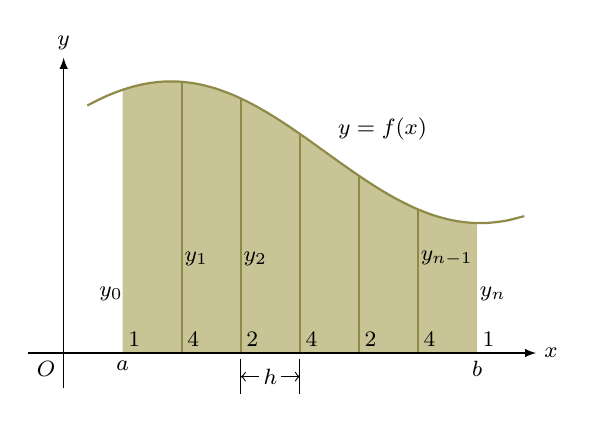
\begin{tikzpicture}[scale=1.5]
            \footnotesize
            \colorlet{ylx}{yellow!50!black}
            \colorlet{yly}{yellow!50!black!50}
    
            \fill [yly] plot [domain=0.5:3.5] (\x,{0.6*sin(1.2*(\x+0.4) r)+1.7}) -- (3.5,0) -- (0.5,0);
            \draw [thick,ylx] plot [domain=0.2:3.9,smooth] (\x,{0.6*sin(1.2*(\x+0.4) r)+1.7});
            \foreach \x in {1,1.5,...,3} {
                \draw [thick,ylx] (\x,0) -- (\x,{0.6*sin(1.2*(\x+0.4) r)+1.7});
            }
            \foreach \x/\s in {0.5/1,1/4,1.5/2,2/4,2.5/2,3/4,3.5/1} {
                \node [above right=-0.5pt,xshift=-0.5pt] at (\x,0) {\s};
            }
            \node [left=-3pt] at (0.5,0.5) {$y_0$};
            \node [right=-2pt] at (1,0.8) {$y_1$};
            \node [right=-2pt] at (1.5,0.8) {$y_2$};
            \node [right=-2pt] at (3,0.8) {$y_{n-1}$};
            \node [right=-2pt] at (3.5,0.5) {$y_n$};
    
            \node [below left] {$O$};
            \node at (2.7,1.9) {$y=f(x)$};
            \node [below] at (0.5,0) {$a$};
            \node [below] at (3.5,0) {$b$};
            \draw [<->] (1.5,-0.2) -- node[fill=white,inner sep=1.5pt]{$h$} (2,-0.2);
            \draw (1.5,-0.05) -- (1.5,-0.35) (2,-0.05) -- (2,-0.35);
    
            \draw [-latex] (-0.3,0) -- (4,0) node[right]{$x$};
            \draw [-latex] (0,-0.3) -- (0,2.5) node[above]{$y$};
        \end{tikzpicture}
        \caption{Simpson's rule.}
        \label{fig:SimpsonsRule}
    \end{figure}
    \begin{itemize}
        \item Simpson's rule approximates the curve via parabolas, which can be uniquely defined by three points and have a nice formula for the area underneath them.
        \item We now derive Simpson's rule.
        \begin{itemize}
            \item Suppose we wish to approximate the area under the part of the curve from $x_i$ to $x_{i+2}$ in Figure \ref{fig:SimpsonsRule}. We know that there exists some parabola intersecting $(x_i,y_0)$, $(x_{i+1},y_1)$, and $(x_{i+2},y_2)$. However, for the sake of simplifying the algebra, we choose to consider the parabola intersecting $(-h,y_0)$, $(0,y_1)$, and $(h,y_2)$ (the area under both parabolas will be equivalent since $x_{i+1}-x_i=h$). Let this translated parabola be called $Ax^2+Bx+C$ for some $A,B,C\in\R$. Then the area underneath this parabola $A_p$ can be described by the following.
            \begin{align*}
                A_p &= \int_{-h}^h\left( Ax^2+Bx+C \right)\dd{x}\\
                &= \frac{2Ah^3}{3}+2Ch
            \end{align*}
            \item We know that the area underneath this parabola is dependent only on $h$, $y_0$, $y_1$, and $y_2$. Thus, we look to express $A,C$ from the integral in terms of $h,y_0,y_1,y_2$. To accomplish this, we will use the facts that
            \begin{align*}
                y_0 &= Ah^2-Bh+C\\
                y_1 &= C\\
                y_2 &= Ah^2+Bh+C
            \end{align*}
            We can now see that $C=y_1$, so all that's left is to solve for $A$. This can be done by adding the first and third equations, substituting, and solving as follows.
            \begin{align*}
                y_0+y_2 &= 2Ah^2+2C\\
                2Ah^2 &= y_0+y_2-2y_1\\
                A &= \frac{y_0-2y_1+y_2}{2h^2}
            \end{align*}
            \item Thus, we can reformulate the area under the parabola as follows.
            \begin{align*}
                A_p &= \frac{2h^3}{3}\cdot\frac{y_0-2y_1+y_2}{2h^2}+2y_1h\\
                &= \frac{h}{3}(y_0+4y_1+y_2)
            \end{align*}
            \item \dq{Simpson's rule follows from applying this result to successive pieces of the curve $y=f(x)$ between $x=a$ and $x=b$. Each separate piece of the curve, covering an $x$-subinterval of width $2h$, is approximated by an arc of a parabola through its ends and its mid-point. The area under each parabolic arc is then given by an expression like [the above] and the results are added to give [the following]}{309}
            \begin{align*}
                A_S &= \frac{h}{3}((y_0+4y_1+y_2)+(y_2+4y_3+y_4)+\cdots+(y_{n-2}+4y_{n-1}+y_n))\\
                &= \frac{h}{3}(y_0+4y_1+2y_2+4y_3+2y_4+\cdots+2y_{n-2}+4y_{n-1}+y_n)
            \end{align*}
        \end{itemize}
        \item Note that the number of subdivisions must be an even integer.
    \end{itemize}
    \item To find the error in a Simpson's rule approximation, use the fact\footnote{A proof of this fact is a topic best left until Analysis. The framework for such a proof may be found on \cite[146]{bib:Olmsted}.} that \dq{if $f$ is continuous on $[a,b]$ and four times differentiable on $(a,b)$, then there is a number $c$ between $a$ and $b$ such that [the following holds]}{310}
    \begin{equation*}
        \int_a^b f(x)\dd{x} = A_S-\frac{b-a}{180}f^{(4)}(c)\cdot h^4
    \end{equation*}
\end{itemize}




\end{document}